\documentclass[conference]{IEEEtran}
\IEEEoverridecommandlockouts

\usepackage{cite}
\usepackage{amsmath,amssymb,amsfonts}
\usepackage{algorithmic}
\usepackage{graphicx}
\usepackage{textcomp}
\usepackage{xcolor}
\def\BibTeX{{\rm B\kern-.05em{\sc i\kern-.025em b}\kern-.08em
    T\kern-.1667em\lower.7ex\hbox{E}\kern-.125emX}}

\begin{document}

\title{Assignment 2}

\author{Tingjun Yuan}

\maketitle

\begin{abstract}
This assignment is mainly based on the knowledge of Attention Mechanisms and
Graph Neural Networks (GNN). The dataset is generally based on a pedestrian
trajectory recorded in a mall. The models trained in the assignment predict
the positions of the pedestrians. This assignment first trains a GNN model
according to a tutorial, but reimplemented with PyTorch. After training, the
model is evaluated with the main squared error (MSE), the mean Euclidean
distance, and the plot graphs. Next, the model is reexamined by tuning
hyperparameters, trying a deeper embedding, and replacing the learned attention
mechanism. This report shows the results of the model evaluation.
\end{abstract}

\section{Result and Evaluation}

\subsection*{Task 1}

This task preprocesses the data, defines the classes for layers and training
logic, trains the model, and evaluates it by calculating the mean squared error
(MSE) and visualizing the differences between prediction and real future
positions. This step follows the tutorial \cite{cite:tut} and rewrites the code
using PyTorch, another deep learning library which is more compatible with the
experiment environment.

The hyperparameters for the training is as follows:

\begin{verbatim}
    hidden_units=100,
    num_heads=8,
    num_layers=3,
    output_dim=2,
    num_epochs=100,
    learning_rate=1e-3,
\end{verbatim}

After training the model for 100 epochs, the training MSE is \textbf{0.4871},
and the test mean Euclidean distance is \textbf{0.2455}. In addition, one of
the scenes is randomly chosen from the test set to perform evaluation by
visualizing the coordinates. The result is shown in Figure~\ref{fig:visual1}.

\begin{figure}[htbp]
    \centering
    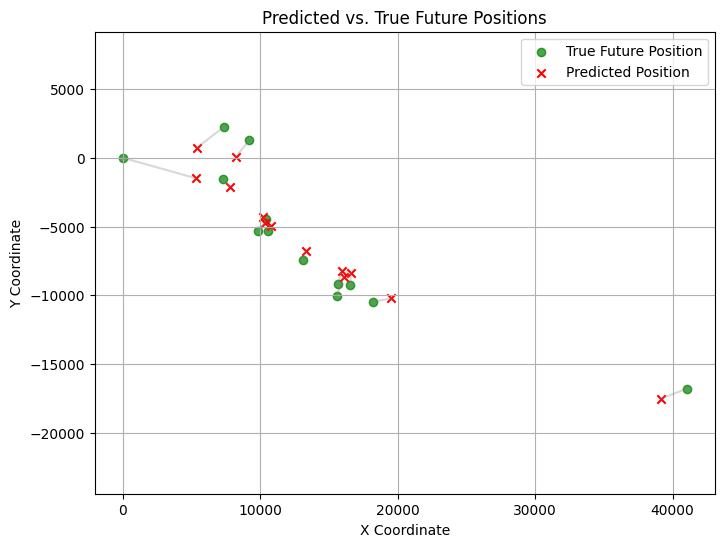
\includegraphics[width=0.8\linewidth]{figvisual1.png}
    \caption{Visualization on the Original Model}
    \label{fig:visual1}
\end{figure}

\subsection*{Task 2}

This task consists of two parts: performing hyperparameter tuning of the number
of attention heads, and trying a deeper embedding of the node features.
Compared with the code provided in Task 1, these parts tried different numbers
of heads: one of them is \texttt{num\_heads=32} (greater than the original), the
other is \texttt{num\_heads=4} (less than the original). The result is shown in
Table~\ref{tab:nh}, the visualization that uses the same scene described above
but applies for \texttt{num\_heads=16} is shown in Figure~\ref{fig:visual2}.
More figures can be seen in the Notebook.

\begin{table}[htbp]
    \caption{Evaluation Result of Different Numbers of Heads}
    \begin{center}
    \begin{tabular}{|c|c|c|}
    \hline
    \textbf{Num of Heads} & \textbf{Train MSE} & \textbf{Test Mean Euclidean Dist} \\
    \hline
    4 & 0.2523 & 0.2159 \\
    \hline
    8\textsuperscript{*} & 0.4871 & 0.2455 \\
    \hline
    16 & 0.5456 & 0.1362 \\
    \hline
    32 & 0.8346 & 0.1375 \\
    \hline

    \multicolumn{3}{l}{\textsuperscript{*}Already done in Task 1, repeated here
        for comparasion}
    \end{tabular}
    \label{tab:nh}
    \end{center}
\end{table}

\begin{figure}[htbp]
    \centering
    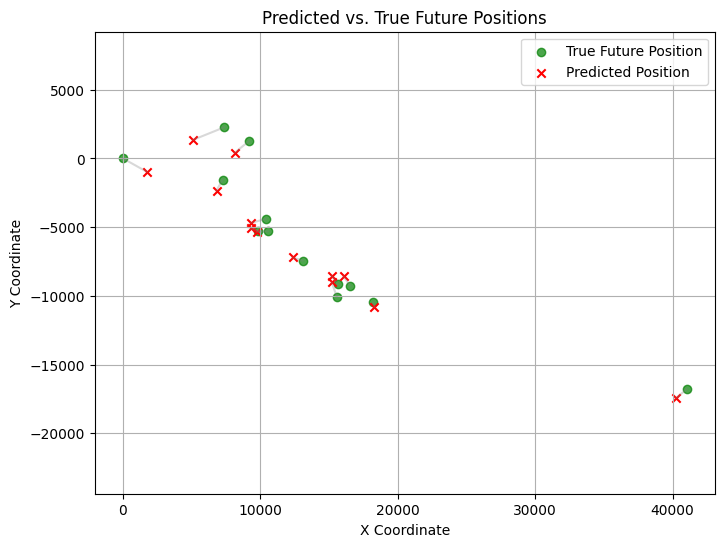
\includegraphics[width=0.8\linewidth]{figvisual2.png}
    \caption{Visualization with num\_heads = 16}
    \label{fig:visual2}
\end{figure}

\subsection*{Task 3}

This task replaces the learned attention mechanism with an attention mechanism
based on the Cosine similarity between node vectors. The modification is based
on Task 2. After training the modified model with the same hyperparameters as
those in Task 1, the training MSE becomes \textbf{0.1885}, and the test mean
Euclidean distance becomes \textbf{0.1078}. The visualization for the scene
that applies this graph is shown in Figure~\ref{fig:visual3}.

\begin{figure}[htbp]
    \centering
    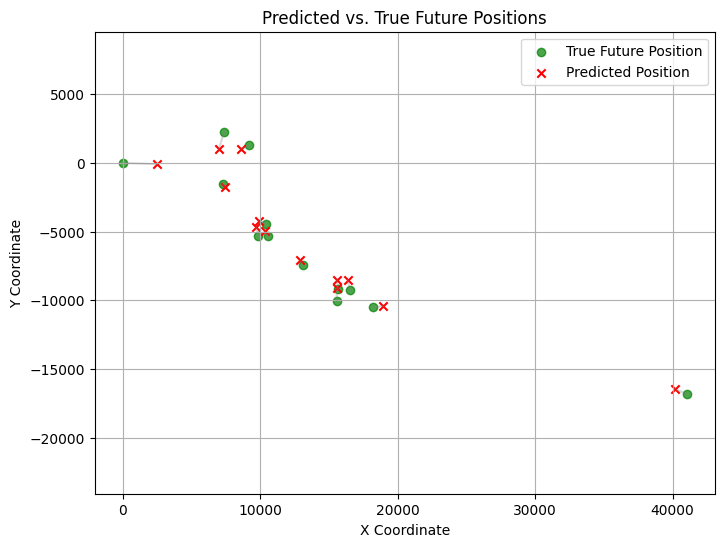
\includegraphics[width=0.8\linewidth]{figvisual3.png}
    \caption{Visualization with Cosine similarity-based attention mechanism}
    \label{fig:visual3}
\end{figure}

\section{Discussion and Conclusion}



\begin{thebibliography}{00}
\bibitem{cite:tut} A. Kensert, “Graph attention network (GAT) for node
    classification,” 2021, Keras. [Online]. Available:
    https://keras.io/examples/graph/gat\_node\_classification/
\end{thebibliography}

\end{document}
